% !TeX program = xelatex
\documentclass[a4paper,10pt]{article}

% ============================================================================
% ១. កញ្ចប់បណ្ណាល័យ និងការកំណត់ទំព័រ (Packages & Page Setup — តាមគំរូ ls_plan.tex)
% ============================================================================
\usepackage[a4paper, left=0.95cm, right=0.95cm, top=0.85cm, bottom=0.92cm, footskip=0.52cm]{geometry}
\usepackage{amsmath}
\usepackage{unicode-math}
\usepackage{fontspec}
\usepackage{longtable, array, multirow, colortbl}
\usepackage[table]{xcolor}
\usepackage{enumitem}
\usepackage{pifont}
\usepackage{fancyhdr}
\usepackage{tikz}
\usetikzlibrary{calc, arrows.meta, decorations.pathreplacing, patterns, positioning, babel}

\makeatletter
\let\@expl@@@mark@update@singlecol@structures@@\relax
\makeatother

% --- ប្រព័ន្ធស្វែងរកទីតាំងពុម្ពអក្សរស្វ័យប្រវត្តិ (Windows Local + Cloud Repo fonts/) ---
\providecommand{\NGSFindFonts}{%
  \IfFileExists{C:/Windows/Fonts/cambria.ttc}{%
    \def\NGSSysPath{C:/Windows/Fonts/}%
    \def\NGSUserPath{C:/Users/KIT/AppData/Local/Microsoft/Windows/Fonts/}%
  }{%
    \IfFileExists{./fonts/KhmerOSsiemreap.ttf}{\def\NGSSysPath{./fonts/}\def\NGSUserPath{./fonts/}}{%
    \IfFileExists{../fonts/KhmerOSsiemreap.ttf}{\def\NGSSysPath{../fonts/}\def\NGSUserPath{../fonts/}}{%
    \IfFileExists{../../fonts/KhmerOSsiemreap.ttf}{\def\NGSSysPath{../../fonts/}\def\NGSUserPath{../../fonts/}}{%
    \IfFileExists{../../../fonts/KhmerOSsiemreap.ttf}{\def\NGSSysPath{../../../fonts/}\def\NGSUserPath{../../../fonts/}}{%
    \IfFileExists{../../../../fonts/KhmerOSsiemreap.ttf}{\def\NGSSysPath{../../../../fonts/}\def\NGSUserPath{../../../../fonts/}}{%
    \IfFileExists{../../../../../fonts/KhmerOSsiemreap.ttf}{\def\NGSSysPath{../../../../../fonts/}\def\NGSUserPath{../../../../../fonts/}}{%
    \IfFileExists{../../../../../../fonts/KhmerOSsiemreap.ttf}{\def\NGSSysPath{../../../../../../fonts/}\def\NGSUserPath{../../../../../../fonts/}}{%
      \def\NGSSysPath{../../../../../../../fonts/}\def\NGSUserPath{../../../../../../../fonts/}%
    }}}}}}}%
  }%
}
\NGSFindFonts

% ============================================================================
% ២. កំណត់ពុម្ពអក្សរ (Fonts — តាមគំរូ ls_plan.tex)
% ============================================================================
\setmathfont[Path={\NGSSysPath}, FontIndex=1, Scale=1.02]{cambria.ttc}
\defaultfontfeatures{Ligatures=TeX}

\setmainfont[
  Path={\NGSUserPath},
  Extension=.ttf,
  Script=Khmer,
  BoldFont={KhmerOSsiemreap},
  BoldFeatures={FakeBold=1.8},
  ItalicFont={KhmerOSsiemreap},
  ItalicFeatures={FakeSlant=0.25},
  BoldItalicFont={KhmerOSsiemreap},
  BoldItalicFeatures={FakeBold=1.8, FakeSlant=0.25}
]{KhmerOSsiemreap}

\newfontfamily\muol[Path={\NGSUserPath}, Extension=.ttf, Script=Khmer]{KhmerOSmuollight}
\newfontfamily\Tacteing[Path={\NGSUserPath}, Extension=.TTF]{TACTENG}
\newfontfamily\TimesEn[Path={\NGSSysPath}, Extension=.ttf, BoldFont={timesbd}, ItalicFont={timesi}, BoldItalicFont={timesbi}]{times}
\newfontfamily\CalibriFont[Path={\NGSSysPath}, Extension=.ttf]{calibri}
\newfontfamily\CourierCirc[Path={\NGSSysPath}, Extension=.ttf]{cour}

\XeTeXlinebreaklocale "km"
\XeTeXlinebreakskip = 0pt plus 1pt minus 0.1pt

% ============================================================================
% ៣. ពណ៌ និងការតុបតែង (Colors & Styles)
% ============================================================================
\definecolor{stepbg}{HTML}{D9D9D9}
\definecolor{headgray}{HTML}{E6E6E6}
\definecolor{emphred}{HTML}{C00000}

\pagestyle{fancy}
\fancyhf{}
\renewcommand{\headrulewidth}{0pt}
\fancyfoot[R]{\CalibriFont\fontsize{9pt}{11pt}\selectfont\thepage}

\setlength{\parindent}{0pt}
\setlength{\parskip}{0pt}
\setlength{\tabcolsep}{4.5pt}
\setlength{\LTpre}{2pt}
\setlength{\LTpost}{2pt}

\newcolumntype{L}[1]{>{\raggedright\arraybackslash}p{#1}}
\newcolumntype{C}[1]{>{\centering\arraybackslash}p{#1}}

% ============================================================================
% ៤. ពាក្យបញ្ជាជំនួយ (Helper Macros)
% ============================================================================
\newcommand{\en}[1]{{\TimesEn #1}}
\newcommand{\enbf}[1]{{\TimesEn\bfseries #1}}
\newcommand{\khmflourish}{{\Tacteing\fontsize{15pt}{15pt}\selectfont 3}}
\newcommand{\wcirc}{{\CourierCirc\fontsize{9.5pt}{11pt}\selectfont o}}
\newcommand{\ditem}{{\fontsize{7.5pt}{10pt}\selectfont\ding{117}}\ }
\newcommand{\fiveE}[1]{\textcolor{emphred}{\CalibriFont\bfseries #1}}
\newcommand{\redsub}[1]{\textcolor{emphred}{#1}}
\newcommand{\timenote}[1]{\textcolor{emphred}{\textit{#1}}}
\newcommand{\stepheader}[1]{\multicolumn{3}{|c|}{\cellcolor{stepbg}\muol #1} \\ \hline}
\newcommand{\cfig}[1]{{\centering\vspace{3pt}#1\vspace{3pt}\par}}
\newcommand{\cnum}[1]{\mbox{\fontsize{10.5pt}{12pt}\selectfont\ding{\numexpr181+#1\relax}}}
\newcommand{\unit}[1]{\,\text{\en{#1}}}
\newcommand{\riel}{\,\text{៛}}
\newcommand{\graybox}[1]{\colorbox{headgray}{\strut #1}}

% ============================================================================
% ៥. រូបភាព TikZ ស-ខ្មៅ សម្រាប់បង្រៀនលើក្ដារខៀន និងសន្លឹកកិច្ចការ (B&W Diagrams)
% ============================================================================

% ១. E1 Engage: អន្ទាក់ច្រឡំបូកនិទស្សន្តពេលបូកឯកធាដូចគ្នា 5x^2 + 3x^2
\newcommand{\figEngageALGFiveTwo}{%
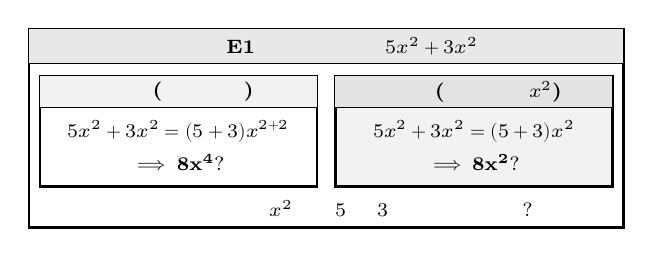
\begin{tikzpicture}[x=1cm, y=1cm, every node/.style={font=\scriptsize, text=black}]
  \draw[black, line width=0.9pt] (0,0) rectangle (7.55,2.52);
  \fill[gray!18] (0,2.08) rectangle (7.55,2.52);
  \draw[black, line width=0.6pt] (0,2.08) -- (7.55,2.08);
  \node at (3.775,2.30) {\textbf{បេសកកម្ម \en{E1}៖ គណនាផលបូកឯកធាដូចគ្នា $5x^2 + 3x^2$}};

  % Student A
  \draw[black, line width=0.8pt] (0.14,0.52) rectangle (3.66,1.92);
  \fill[gray!10] (0.14,1.52) rectangle (3.66,1.92);
  \draw[black, line width=0.5pt] (0.14,1.52) -- (3.66,1.52);
  \node at (1.90,1.72) {\textbf{សិស្ស ក (បូកទាំងស្វ័យគុណ)}};
  \node at (1.90,1.22) {$5x^2 + 3x^2 = (5+3)x^{2+2}$};
  \node at (1.90,0.82) {$\implies \mathbf{8x^4}$?};

  % Student B
  \draw[black, line width=0.95pt, fill=gray!10] (3.89,0.52) rectangle (7.41,1.92);
  \fill[gray!22] (3.89,1.52) rectangle (7.41,1.92);
  \draw[black, line width=0.55pt] (3.89,1.52) -- (7.41,1.52);
  \node at (5.65,1.72) {\textbf{សិស្ស ខ (រក្សាផ្នែកអថេរ $x^2$)}};
  \node at (5.65,1.22) {$5x^2 + 3x^2 = (5+3)x^2$};
  \node at (5.65,0.82) {$\implies \mathbf{8x^2}$?};

  \node at (3.775,0.24) {\textbf{សំណួរគន្លឹះ៖} បើបូកការេផ្ទៃ $x^2$ ចំនួន $5$ និង $3$ បន្ទះ តើបានការេប្រភេទណា?};
\end{tikzpicture}}

% ២. E2 Explore: គំរូផ្ទៃក្រឡាបូកឯកធា b+2b+3b=6b និងគុណចែកឯកធា (5x)(2x), 16xy^2/(4y)
\newcommand{\figAreaOpsALGFiveTwo}{%
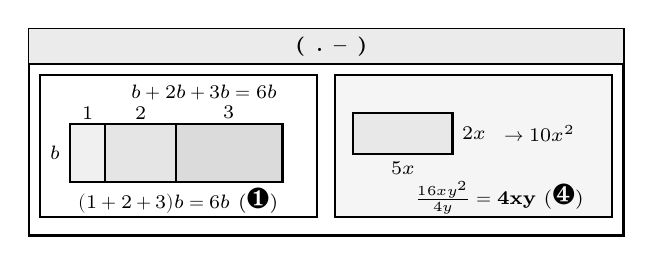
\begin{tikzpicture}[x=1cm, y=1cm, every node/.style={font=\scriptsize, text=black}]
  \draw[black, line width=0.9pt] (0,0) rectangle (7.55,2.62);
  \fill[gray!16] (0,2.18) rectangle (7.55,2.62);
  \draw[black, line width=0.6pt] (0,2.18) -- (7.55,2.18);
  \node at (3.775,2.40) {\textbf{គំរូផ្ទៃក្រឡាចតុកោណកែង (ទំ.៥៣--៥៥)៖ បូក គុណ និងចែកឯកធា}};

  % Left: b + 2b + 3b = 6b
  \draw[black, line width=0.8pt] (0.14,0.24) rectangle (3.66,2.04);
  \node at (1.90,1.82) {\textbf{បូកផ្ទៃ៖ $b + 2b + 3b = 6b$}};
  \draw[black, line width=0.8pt, fill=gray!12] (0.52,0.68) rectangle (0.97,1.42);
  \draw[black, line width=0.8pt, fill=gray!20] (0.97,0.68) rectangle (1.87,1.42);
  \draw[black, line width=0.8pt, fill=gray!28] (1.87,0.68) rectangle (3.22,1.42);
  \node at (0.34,1.05) {$b$};
  \node at (0.745,1.56) {$1$};
  \node at (1.42,1.56) {$2$};
  \node at (2.545,1.56) {$3$};
  \node at (1.90,0.44) {$(1+2+3)b = 6b$ (\cnum{1})};

  % Right: Garden 5x * 2x & Pond 16xy^2 / 4y
  \draw[black, line width=0.8pt, fill=gray!8] (3.89,0.24) rectangle (7.41,2.04);
  \node at (5.65,1.82) {\textbf{សួនច្បារ និងស្រះទឹក}};
  \draw[black, line width=0.8pt, fill=gray!18] (4.12,1.04) rectangle (5.38,1.56);
  \node at (4.75,0.85) {$5x$};
  \node at (5.65,1.30) {$2x$};
  \node[anchor=west] at (5.92,1.30) {$\to 10x^2$};
  \node at (5.65,0.48) {ស្រះទឹក៖ $\tfrac{16xy^2}{4y} = \mathbf{4xy}$ (\cnum{4})};
\end{tikzpicture}}

% ៣. E3 Explain: តារាងប្រៀបធៀបក្បួនបូក/ដក vs. គុណ/ចែកឯកធា
\newcommand{\figRuleCompareALGFiveTwo}{%
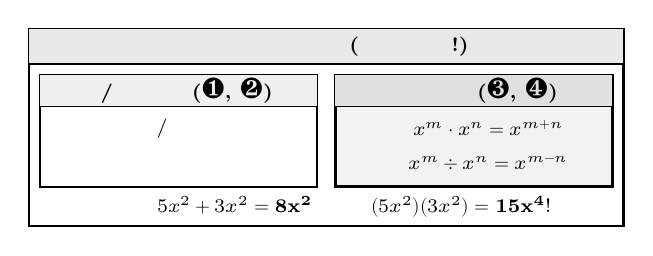
\begin{tikzpicture}[x=1cm, y=1cm, every node/.style={font=\scriptsize, text=black}]
  \draw[black, line width=0.9pt] (0,0) rectangle (7.55,2.50);
  \fill[gray!18] (0,2.06) rectangle (7.55,2.50);
  \draw[black, line width=0.6pt] (0,2.06) -- (7.55,2.06);
  \node at (3.775,2.28) {\textbf{ប្រៀបធៀបក្បួនប្រមាណវិធីលើឯកធា (កុំច្រឡំឆ្លងក្បួន!)}};

  % Left: Add/Sub like monomials
  \draw[black, line width=0.8pt] (0.14,0.50) rectangle (3.66,1.92);
  \fill[gray!12] (0.14,1.52) rectangle (3.66,1.92);
  \draw[black, line width=0.55pt] (0.14,1.52) -- (3.66,1.52);
  \node at (1.90,1.72) {\textbf{បូក/ដកឯកធាដូចគ្នា (\cnum{1}, \cnum{2})}};
  \node at (1.90,1.24) {បូក/ដក\textbf{តែមេគុណ}};
  \node at (1.90,0.80) {\textbf{រក្សាផ្នែកអថេរដដែល}};

  % Right: Multiply & Divide monomials
  \draw[black, line width=0.95pt, fill=gray!10] (3.89,0.50) rectangle (7.41,1.92);
  \fill[gray!24] (3.89,1.52) rectangle (7.41,1.92);
  \draw[black, line width=0.6pt] (3.89,1.52) -- (7.41,1.52);
  \node at (5.65,1.72) {\textbf{គុណ និងចែកឯកធា (\cnum{3}, \cnum{4})}};
  \node at (5.65,1.24) {គុណ៖ $x^m \cdot x^n = x^{m+n}$};
  \node at (5.65,0.80) {ចែក៖ $x^m \div x^n = x^{m-n}$};

  \node at (3.775,0.24) {\textbf{ប្រៀបធៀប៖} $5x^2 + 3x^2 = \mathbf{8x^2}$ \quad ឯ \quad $(5x^2)(3x^2) = \mathbf{15x^4}$!};
\end{tikzpicture}}

% ៤. E4 Elaborate: ប្លង់ភូមិគ្រឹះ 18a x 12a = 216a^2 និងលំហាត់គំរូចែកឯកធា
\newcommand{\figMansionALGFiveTwo}{%
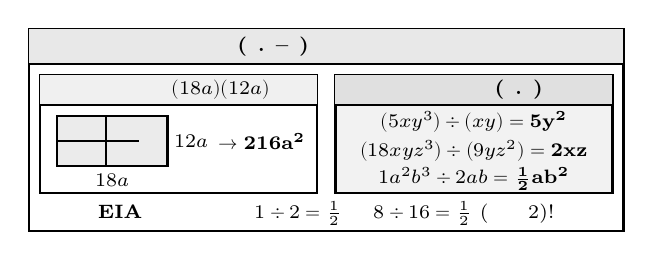
\begin{tikzpicture}[x=1cm, y=1cm, every node/.style={font=\scriptsize, text=black}]
  \draw[black, line width=0.9pt] (0,0) rectangle (7.55,2.56);
  \fill[gray!18] (0,2.12) rectangle (7.55,2.56);
  \draw[black, line width=0.6pt] (0,2.12) -- (7.55,2.12);
  \node at (3.775,2.34) {\textbf{លំហាត់គំរូ (ទំ.៥៤--៥៦)៖ ប្លង់ភូមិគ្រឹះ និងការចែកឯកធា}};

  % Left: Floor plan 18a by 12a
  \draw[black, line width=0.8pt] (0.14,0.48) rectangle (3.66,1.98);
  \fill[gray!12] (0.14,1.60) rectangle (3.66,1.98);
  \draw[black, line width=0.55pt] (0.14,1.60) -- (3.66,1.60);
  \node at (1.90,1.79) {\textbf{ប្លង់ភូមិគ្រឹះ $(18a)(12a)$}};
  \draw[black, line width=0.85pt, fill=gray!16] (0.36,0.82) rectangle (1.76,1.46);
  \draw[black, line width=0.5pt] (0.98,0.82) -- (0.98,1.46);
  \draw[black, line width=0.5pt] (0.36,1.14) -- (1.40,1.14);
  \node at (1.06,0.64) {$18a$};
  \node at (2.06,1.14) {$12a$};
  \node at (2.96,1.14) {$\to \mathbf{216a^2}$};

  % Right: Division model examples
  \draw[black, line width=0.95pt, fill=gray!10] (3.89,0.48) rectangle (7.41,1.98);
  \fill[gray!24] (3.89,1.60) rectangle (7.41,1.98);
  \draw[black, line width=0.6pt] (3.89,1.60) -- (7.41,1.60);
  \node at (5.65,1.79) {\textbf{គំរូវិធីចែកឯកធា (ទំ.៥៦)}};
  \node at (5.65,1.38) {$(5xy^3)\div(xy) = \mathbf{5y^2}$};
  \node at (5.65,1.02) {$(18xyz^3)\div(9yz^2) = \mathbf{2xz}$};
  \node at (5.65,0.66) {$1a^2b^3 \div 2ab = \mathbf{\tfrac{1}{2}ab^2}$};

  \node at (3.775,0.22) {\textbf{\en{EIA}៖} ចែកមេគុណតាមលំដាប់ $1 \div 2 = \tfrac{1}{2}$ និង $8 \div 16 = \tfrac{1}{2}$ (មិនមែន $2$)!};
\end{tikzpicture}}

% ៥. E5 Evaluate: ជម្រើសវិនិច្ឆ័យ A-D គណនា (-4a^2b^3)(3ab^2)
\newcommand{\figExitALGFiveTwo}{%
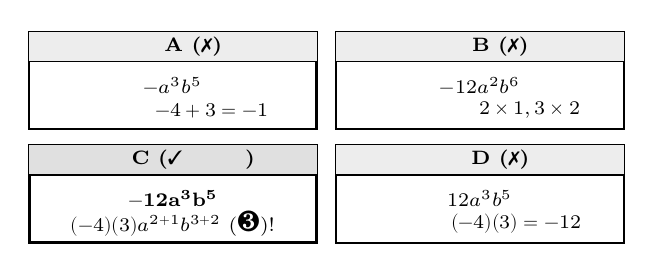
\begin{tikzpicture}[x=1cm, y=1cm, every node/.style={font=\scriptsize, text=black}]
  % Choice A
  \draw[black, line width=0.8pt] (0,1.44) rectangle (3.65,2.68);
  \fill[gray!14] (0,2.30) rectangle (3.65,2.68);
  \draw[black, line width=0.5pt] (0,2.30) -- (3.65,2.30);
  \node at (1.825,2.49) {\textbf{ជម្រើស \en{A} (\ding{55})}};
  \node at (1.825,2.00) {$-a^3b^5$};
  \node at (1.825,1.68) {ច្រឡំបូកមេគុណ $-4+3=-1$};

  % Choice B
  \draw[black, line width=0.8pt] (3.90,1.44) rectangle (7.55,2.68);
  \fill[gray!14] (3.90,2.30) rectangle (7.55,2.68);
  \draw[black, line width=0.5pt] (3.90,2.30) -- (7.55,2.30);
  \node at (5.725,2.49) {\textbf{ជម្រើស \en{B} (\ding{55})}};
  \node at (5.725,2.00) {$-12a^2b^6$};
  \node at (5.725,1.68) {ច្រឡំគុណនិទស្សន្ត $2\times 1, 3\times 2$};

  % Choice C (Correct)
  \draw[black, line width=1.05pt] (0,0) rectangle (3.65,1.24);
  \fill[gray!24] (0,0.86) rectangle (3.65,1.24);
  \draw[black, line width=0.6pt] (0,0.86) -- (3.65,0.86);
  \node at (1.825,1.05) {\textbf{ជម្រើស \en{C} (\ding{51} ត្រឹមត្រូវ)}};
  \node at (1.825,0.56) {$\mathbf{-12a^3b^5}$};
  \node at (1.825,0.24) {$(-4)(3)a^{2+1}b^{3+2}$ (\cnum{3})!};

  % Choice D
  \draw[black, line width=0.8pt] (3.90,0) rectangle (7.55,1.24);
  \fill[gray!14] (3.90,0.86) rectangle (7.55,1.24);
  \draw[black, line width=0.5pt] (3.90,0.86) -- (7.55,0.86);
  \node at (5.725,1.05) {\textbf{ជម្រើស \en{D} (\ding{55})}};
  \node at (5.725,0.56) {$12a^3b^5$};
  \node at (5.725,0.24) {ភ្លេចសញ្ញាដក $(-4)(3) = -12$};
\end{tikzpicture}}

\begin{document}
\fontsize{10pt}{15.2pt}\selectfont

% ============================================================================
% ក្បាលរដ្ឋបាល (Administrative Header — តាមគំរូ ls_plan.tex)
% ============================================================================
{\centering
  {\muol\fontsize{11pt}{16pt}\selectfont ព្រះរាជាណាចក្រកម្ពុជា\par}
  {\muol\fontsize{11pt}{16pt}\selectfont ជាតិ សាសនា ព្រះមហាក្សត្រ\par}
  \vspace{-3pt}{\khmflourish\par}
}

\vspace{1pt}
{\muol\fontsize{10pt}{15.5pt}\selectfont
មន្ទីរអប់រំ យុវជន និងកីឡា ខេត្តកំពង់ធំ\par
ការិយាល័យអប់រំ យុវជន និងកីឡា ស្រុកកំពង់ស្វាយ\par
អនុវិទ្យាល័យព្រះក្រសាំង\par}

\vspace{2pt}
{\centering{\muol\fontsize{11.5pt}{17pt}\selectfont កិច្ចតែងការបង្រៀន\par}}
\vspace{2pt}

% --- ព័ត៌មានទូទៅ ---
{\hspace*{2.8cm}\renewcommand{\arraystretch}{1.08}
\begin{tabular}{@{}l@{\hspace{0.35cm}}p{2.9cm}@{\hspace{0.15cm}}c@{\hspace{0.25cm}}l@{}}
  - & មុខវិជ្ជា & : & គណិតវិទ្យា ថ្នាក់ទី៨ (ពីជគណិត) \\
  - & ចំណងជើងមេរៀន & : & មេរៀនទី៥៖ កន្សោមពីជគណិត \\
  - & ចំណងជើងរង & : & ១.៤ បូកនិងដកឯកធាដូចគ្នា, ១.៥ វិធីគុណឯកធា និង ១.៦ វិធីចែកឯកធា \\
  - & រយៈពេល & : & ១ ម៉ោងសិក្សា (៥០ នាទី) \\
  - & បង្រៀនដោយ & : & ហុក ប៊ុនថែន \\
  - & កាលបរិច្ឆេទ & : & ថ្ងៃសៅរ៍ ទី៥ ខែធ្នូ ឆ្នាំ២០២៦ \\
\end{tabular}\par}

\vspace{2pt}

% --- I. វត្ថុបំណង ---
{\muol\fontsize{10pt}{15.5pt}\selectfont \enbf{I.} វត្ថុបំណង\par}
\vspace{1pt}
{\renewcommand{\arraystretch}{1.10}
\begin{tabular}{@{}p{0.55cm}@{}p{2.35cm}@{\hspace{0.15cm}}c@{\hspace{0.25cm}}p{14.95cm}@{}}
  \hfill\wcirc\hspace{0.2cm} & វិជ្ជាសម្បទា & : & សិស្សប្រាប់ក្បួនបូកនិងដកឯកធាដូចគ្នា វិធីគុណឯកធា និងវិធីចែកឯកធានឹងឯកធាបានត្រឹមត្រូវតាមសៀវភៅសិក្សាគោល (ទំ.៥៣--៥៦) ។ \\
  \hfill\wcirc\hspace{0.2cm} & បំណិនសម្បទា & : & សិស្សគណនាផលបូក ផលដក ផលគុណ និងផលចែកឯកធា (រួមទាំងបញ្ហាផ្ទៃក្រឡាសួនច្បារ ប្លង់ភូមិគ្រឹះ និងស្រះទឹក) លើសន្លឹកកិច្ចការបានត្រឹមត្រូវ ។ \\
  \hfill\wcirc\hspace{0.2cm} & ចរិយាសម្បទា & : & សិស្សមានទម្លាប់ផ្ទៀងផ្ទាត់សញ្ញាមេគុណនិងនិទស្សន្តយ៉ាងប្រុងប្រយ័ត្ន មិនភាន់ច្រឡំក្បួនបូកឯកធាដូចគ្នាជាមួយក្បួនគុណឯកធា ។ \\
\end{tabular}\par}

\vspace{2pt}

% --- II. សម្ភារៈឧបទេស ---
{\muol\fontsize{10pt}{15.5pt}\selectfont \enbf{II.} សម្ភារៈឧបទេស\par}
\vspace{1pt}
\hspace*{0.55cm}$\bullet$\ សៀវភៅសិក្សាគោលថ្នាក់ទី៨ (ទំ.៥៣--៥៦, ៧២) ក្ដារខៀន ដីស/ហ្វឺត បន្ទាត់ត្រង់ និង\textbf{សន្លឹកកិច្ចការសិស្សបំពេញចន្លោះ ស-ខ្មៅ} (កូដ \en{ALG52} ទំព័រ ១--២ សម្រាប់សិស្ស និងទំព័រ ៣ ប្លង់ក្ដារខៀន/ចម្លើយគ្រូ — គ្មានប្រើ \en{LCD})\par

\vspace{2pt}

% --- III. វិធីសាស្រ្តបង្រៀន ---
{\muol\fontsize{10pt}{15.5pt}\selectfont \enbf{III.} វិធីសាស្រ្តបង្រៀន\par}
\vspace{1pt}
{\renewcommand{\arraystretch}{1.08}
\begin{tabular}{@{}p{0.55cm}@{}p{2.35cm}@{\hspace{0.15cm}}c@{\hspace{0.25cm}}p{14.95cm}@{}}
  \hfill$\bullet$\hspace{0.2cm} & គោលវិធី & : & សិស្សមជ្ឈមណ្ឌល (សន្លឹកកិច្ចការបំពេញចន្លោះជាគោល + ការពិភាក្សាជាក្រុមតូច ៣ នាក់) \\
  \hfill$\bullet$\hspace{0.2cm} & យុទ្ធវិធីបង្រៀន & : & គំរូស្ថាបនានិយម \en{5Es} រួមបញ្ចូល \textbf{គំរូផ្ទៃក្រឡាចតុកោណកែង} និង \textbf{ការប្រៀបធៀបទន្ទឹមគ្នា (\en{Contrasting Cases})} រវាងការបូក និងការគុណឯកធា \\
\end{tabular}\par}

\vspace{2pt}

% --- IV. ដំណើរការបង្រៀន ---
{\muol\fontsize{10pt}{15.5pt}\selectfont \enbf{IV.} ដំណើរការបង្រៀន\par}

{\renewcommand{\arraystretch}{1.15}
\begin{longtable}{|L{5.50cm}|L{7.90cm}|L{4.80cm}|}
\hline
\multicolumn{1}{|c|}{\cellcolor{headgray}\muol សកម្មភាពគ្រូ} &
\multicolumn{1}{c|}{\cellcolor{headgray}\muol ខ្លឹមសារមេរៀន} &
\multicolumn{1}{c|}{\cellcolor{headgray}\muol សកម្មភាពសិស្ស} \\
\hline
\endfirsthead

\hline
\multicolumn{1}{|c|}{\cellcolor{headgray}\muol សកម្មភាពគ្រូ} &
\multicolumn{1}{c|}{\cellcolor{headgray}\muol ខ្លឹមសារមេរៀន} &
\multicolumn{1}{c|}{\cellcolor{headgray}\muol សកម្មភាពសិស្ស} \\
\hline
\endhead

% ==================== ជំហានទី១ (2min) ====================
\stepheader{ជំហានទី១ \enbf{(}រដ្ឋបាលថ្នាក់\enbf{)}}
$\bullet$ ពិនិត្យវត្តមាន អនាម័យ និងសណ្ដាប់ធ្នាប់ថ្នាក់រៀន \par
$\bullet$ រៀបចំក្រុមតូច ៣ នាក់ និងចែក\textbf{សន្លឹកកិច្ចការសិស្ស (\en{ALG52} ទំព័រ ១–២)}
&
$\bullet$ រដ្ឋបាលថ្នាក់ អនាម័យ និងវិន័យសិក្សា \par
$\bullet$ ចែកសន្លឹកកិច្ចការម្នាក់ ១ សន្លឹក សម្រាប់បំពេញតាមដំណាក់កាល \en{E1--E5}
&
$\circ$ ប្រធានថ្នាក់រាយការណ៍វត្តមានសិស្ស \par
$\circ$ ទទួលសន្លឹកកិច្ចការ សរសេរឈ្មោះ និងអង្គុយតាមក្រុម ៣ នាក់ \\
\hline

% ==================== ជំហានទី២ (9min: កំណែ <=3m + រំលឹក 3m + E1 3m) ====================
\stepheader{ជំហានទី២ \enbf{(}កិច្ចការផ្ទះ \enbf{+} ទំនាក់ទំនងមេរៀនថ្មី\enbf{)}}
\ditem \textbf{កំណែកិច្ចការផ្ទះ ($\le\text{\enbf{3\,min}}$)} \par
$\bullet$ ហៅសិស្ស ២ នាក់ឡើងកែប្រតិបត្តិទំ.៥៣ (ង, ច, ឆ) និងលំហាត់ទំ.៧២ \#1 លើក្ដារខៀន
&
{\centering\redsub{កំណែកិច្ចការផ្ទះ (ទំ.៥៣ ង, ច, ឆ និង ទំ.៧២ \#1)}\par}
$\bullet$ \textbf{ទំ.៥៣៖} ង) $21ab^4c \to$ ដឺក្រេ $\mathbf{6}$; \ ច) $3x^2y^3z^4 \to$ ដឺក្រេ $\mathbf{9}$; \ ឆ) $axyz \to$ ដឺក្រេ $\mathbf{4}$ \par
$\bullet$ \textbf{ទំ.៧២ \#1៖} ឯកធាគឺ $\mathbf{\tfrac{x^3}{3}, \ \sqrt{5}ax^2, \ \tfrac{7xy^2}{3}}$ (ឯ $x+2y, \tfrac{a}{x^2}, x(x+y)$ មិនមែនទេ)
&
$\circ$ ផ្ទៀងចម្លើយ និងកែតម្រូវចូលសៀវភៅកិច្ចការផ្ទះ \\[3pt]

\ditem \textbf{រំលឹកមេរៀនទាក់ទង (\enbf{3min})} \par
$\bullet$ សួរ៖ «តើឯកធាដូចគ្នាមានលក្ខណៈដូចម្ដេច? ចុះ $x^m \cdot x^n$ និង $\frac{x^m}{x^n}$ ស្មើអ្វី?»
&
{\centering\redsub{រំលឹកឯកធាដូចគ្នា និងរូបមន្តស្វ័យគុណ}\par}
$\bullet$ ឯកធាដូចគ្នា៖ មានផ្នែកអថេរដូចគ្នាគត់ (ដូចជា $5x^2$ និង $3x^2$) \par
$\bullet$ រូបមន្តស្វ័យគុណ៖ $x^m \cdot x^n = x^{m+n}$ និង $\dfrac{x^m}{x^n} = x^{m-n}\ (x\neq 0)$
&
$\circ$ ឆ្លើយ៖ «ផ្នែកអថេរដូចគ្នា; គុណបូកនិទស្សន្ត ចែកដកនិទស្សន្ត!» \\[3pt]

\fiveE{E1 - Engage (3min)} \timenote{(កុំទាន់ផ្ដល់ចម្លើយ)} \par
\ditem \textbf{បេសកកម្មអន្ទាក់ស្វ័យគុណពេលបូកឯកធា (សន្លឹកកិច្ចការ \en{E1})} \par
$\bullet$ ឱ្យសិស្សអានប្រអប់ \en{E1} ហើយគូសជ្រើសរើសរវាង\textbf{សិស្ស ក} និង\textbf{សិស្ស ខ}
&
\redsub{បេសកកម្ម \en{E1}៖ គណនាផលបូក $5x^2 + 3x^2$ តើស្មើប៉ុន្មាន?} \par
$\bullet$ \textbf{សិស្ស ក} បូកទាំងនិទស្សន្តថា $5x^2 + 3x^2 = 8x^4$! \par
$\bullet$ \textbf{សិស្ស ខ} រាប់ការេផ្ទៃ $x^2$ ចំនួន $5$ បន្ទះ បូក $3$ បន្ទះ ថាស្មើ $8x^2$! តើអ្នកណាត្រូវ?
&
$\circ$ ពិភាក្សាជាគូ និងគូស \ding{51} ក្នុងប្រអប់ \en{E1} លើសន្លឹកកិច្ចការ \\[3pt]

&
\cfig{\figEngageALGFiveTwo}
& \\
\hline

% ==================== ជំហានទី៣ (17min: E2 11m + E3 6m) ====================
\stepheader{ជំហានទី៣ \enbf{(}ខ្លឹមសារមេរៀនថ្មី\enbf{)}}
\fiveE{E2 - Explore (11min)} \par
$\bullet$ សរសេរចំណងជើងរង \textbf{១.៤–១.៦ ប្រមាណវិធីលើឯកធា} លើក្ដារខៀន \par
\ditem \textbf{សកម្មភាព ១៖ បូក និងដកឯកធាដូចគ្នា (ទំ.៥៣–៥៤, \enbf{5min}, \en{E2-A})} \par
$\bullet$ ឱ្យសិស្សបំពេញផលបូកផ្ទៃចតុកោណកែង $b + 2b + 3b$ និងផលដក $5x - 2x$ លើ \en{E2-A}
&
១.៤ ប្រមាណវិធីបូកនិងដកឯកធាដូចគ្នា \par
$\bullet$ \textbf{ឧទាហរណ៍ទី ១ (ទំ.៥៣)៖} ផ្ទៃចតុកោណកែងទាំងបី $b + 2b + 3b = (1+2+3)b = \mathbf{6b}$ \par
$\bullet$ \textbf{ឧទាហរណ៍ទី ២ (ទំ.៥៣)៖} បន្ទះពិជគណិត $5x - 2x = (5-2)x = \mathbf{3x}$ \par
$\bullet$ \textbf{លំហាត់គំរូ (ទំ.៥៤ ក, ខ)៖} $2xy + 5xy = (2+5)xy = \mathbf{7xy}$; \ $3ab^2 + 7ab^2 + ab^2 = (3+7+1)ab^2 = \mathbf{11ab^2}$ (កុំភ្លេច $ab^2 = 1ab^2$!)
&
$\circ$ គណនាឃើញ $6b, 3x, 7xy$ និង $11ab^2$ លើសន្លឹកកិច្ចការ \\[3pt]

\ditem \textbf{សកម្មភាព ២៖ វិធីគុណ និងវិធីចែកឯកធា (ទំ.៥៤–៥៥, \enbf{6min}, \en{E2-B})} \par
$\bullet$ ឱ្យសិស្សគណនាផ្ទៃសួនច្បារ $(5x)(2x)$ និងបណ្ដោយស្រះទឹក $\frac{16xy^2}{4y}$ លើ \en{E2-B}
&
១.៥ វិធីគុណឯកធា \quad និង \quad ១.៦ វិធីចែកឯកធា \par
$\bullet$ \textbf{គុណឯកធា (ទំ.៥៤)៖} ផ្ទៃសួនច្បារ $(5x)(2x) = (5)(2)(x)(x) = \mathbf{10x^2}$; \ ឧ.២៖ $(4x^2yc^4)(3xy^3c) = (4)(3)x^{2+1}y^{1+3}c^{4+1} = \mathbf{12x^3y^4c^5}$ \par
$\bullet$ \textbf{ចែកឯកធា (ទំ.៥៥)៖} បណ្ដោយស្រះទឹក $\dfrac{16xy^2}{4y} = \mathbf{4xy}$; \ ឧ.២៖ $(8x^4y^5)\div(16x^2y^3) = \dfrac{8}{16}x^{4-2}y^{5-3} = \mathbf{\dfrac{1}{2}x^2y^2}$
&
$\circ$ រកឃើញថាគុណឯកធាបូកនិទស្សន្ត ឯចែកឯកធាដកនិទស្សន្ត \\[3pt]

&
\cfig{\figAreaOpsALGFiveTwo}
& \\[3pt]

% --- E3 Explain (6min) ---
\fiveE{E3 - Explain (6min)} \par
$\bullet$ ដឹកនាំសិស្សសង្ខេបក្បួន \textbf{«ជាទូទៅ»} ទាំង ៣ (ទំ.៥៤–៥៥) ដាក់ប្រៀបធៀបគ្នា
&
$\bullet$ \textbf{ក្បួន «ជាទូទៅ» (ទំ.៥៤–៥៥)៖} \par
\hspace*{0.15cm}១) \textbf{បូក/ដកឯកធាដូចគ្នា៖} បូកឬដក\graybox{តែផ្នែកមេគុណ} រួចគុណនឹង\graybox{ផ្នែកអថេរដដែល} \par
\hspace*{0.15cm}២) \textbf{គុណឯកធា៖} ផ្គុំគុណមេគុណនឹងមេគុណ និងផ្នែកអថេរនឹងផ្នែកអថេរ ($x^m \cdot x^n = x^{m+n}$) \par
\hspace*{0.15cm}៣) \textbf{ចែកឯកធា៖} ចែកមេគុណនឹងមេគុណ និងផ្នែកអថេរនឹងផ្នែកអថេរ ($x^m \div x^n = x^{m-n}$)
&
$\circ$ បំពេញប្រអប់ក្បួនទាំង ៣ លើសន្លឹកកិច្ចការ \en{E3} \\[3pt]

$\bullet$ ភ្ជាប់\textbf{ធនាគារហេតុផល \cnum{1}--\cnum{4}} លើក្ដារខៀន និងសន្លឹកកិច្ចការ
&
\textbf{ធនាគារហេតុផល (\en{Warrant Bank})៖} \par
\cnum{1} \textbf{បូក/ដកឯកធាដូចគ្នា៖} $ax^n \pm bx^n = (a\pm b)x^n$ (ហាមបូកនិទស្សន្ត!) \par
\cnum{2} \textbf{មេគុណលាក់មុខ៖} $x^2y = 1x^2y$ និង $-x^2y = -1x^2y$
&
$\circ$ ផ្ទៀងលេខកូដ \cnum{1}--\cnum{2} លើសន្លឹកកិច្ចការ \\[3pt]

&
\cnum{3} \textbf{គុណឯកធា៖} គុណមេគុណ បូកនិទស្សន្តអថេរដូចគ្នា ($x^m \cdot x^n = x^{m+n}$) \par
\cnum{4} \textbf{ចែកឯកធា៖} សរសេរជាប្រភាគ សម្រួលមេគុណ និងដកនិទស្សន្ត ($\tfrac{x^m}{x^n} = x^{m-n}$)
&
$\circ$ ផ្ទៀងលេខកូដ \cnum{3}--\cnum{4} លើសន្លឹកកិច្ចការ \\[3pt]

&
\cfig{\figRuleCompareALGFiveTwo}
& \\
\hline

% ==================== ជំហានទី៤ (20min: E4 10m + E5 10m) ====================
\stepheader{ជំហានទី៤ \enbf{(}ពង្រីកចំណេះដឹង\enbf{)}}
\fiveE{E4 - Elaborate (10min)} \par
\ditem \textbf{លំហាត់គំរូ៖ បូកដក គុណប្លង់ភូមិគ្រឹះ និងចែកឯកធា (ទំ.៥៤–៥៦)} \par
$\bullet$ ឱ្យសិស្សដោះស្រាយលំហាត់គំរូទាំង ៣ ផ្នែកលើសន្លឹកកិច្ចការ \en{E4}
&
{\muol លំហាត់គំរូ} \textbf{(ទំ.៥៤–៥៦)៖} \par
$\bullet$ \textbf{១) បូកដក (ទំ.៥៤ គ, ឃ)៖} $8x^2y^3z - 3x^2y^3z - 7x^2y^3z = (8-3-7)x^2y^3z = \graybox{$-2x^2y^3z$}$; \quad $10x^2y + x^2y - 5x^2y = (10+1-5)x^2y = \graybox{$6x^2y$}$ \par
$\bullet$ \textbf{២) ផ្ទៃក្រឡាប្លង់ភូមិគ្រឹះ (ទំ.៥៥)៖} $A = (18a)(12a) = \graybox{$216a^2$}$ ឯកតាផ្ទៃ \par
$\bullet$ \textbf{៣) ចែកឯកធា (ទំ.៥៦)៖} ក) $(5xy^3)\div(xy) = \mathbf{5y^2}$; \ ខ) $\dfrac{18xyz^3}{9yz^2} = \mathbf{2xz}$; \ គ) $1a^2b^3\div 2ab = \mathbf{\dfrac{1}{2}ab^2}$
&
$\circ$ គណនាបាន $-2x^2y^3z, 6x^2y, 216a^2$ និង $5y^2, 2xz, \tfrac{1}{2}ab^2$ \\[3pt]

&
\cfig{\figMansionALGFiveTwo}
& \\[3pt]

$\bullet$ សួរសំណួរឆ្លុះបញ្ចាំង \textbf{\en{EIA Looking-Back} (1min)}
&
\textbf{\en{EIA Looking-Back}៖} «ហេតុអ្វី $1a^2b^3 \div 2ab$ និង $(8x^4y^5)\div(16x^2y^3)$ មានមេគុណស្មើ $\frac{1}{2}$ មិនមែនស្មើ $2$ ទេ?» ($\to$ ព្រោះតួតំណាងចែក $1$ និង $8$ នៅភាគយក ចែកនឹងតួចែក $2$ និង $16$ នៅភាគបែង បាន $\frac{1}{2}$!)
&
$\circ$ ពន្យល់ថាត្រូវសរសេរជាប្រភាគមុនសម្រួលមេគុណ \\[3pt]

% --- E5 Evaluate (10min) ---
\fiveE{E5 - Evaluate (10min)} \par
\ditem \textbf{ប្រតិបត្តិជាក្រុមតូច ៣ នាក់ (4min, សន្លឹកកិច្ចការ \en{E5})} \par
$\bullet$ ឱ្យសិស្សគណនាប្រតិបត្តិទំ.៥៤ (ក, គ) ទំ.៥៥ (ក) និងទំ.៥៦ (ឃ)
&
{\muol លំហាត់ប្រតិបត្តិ} \textbf{(ទំ.៥៤–៥៦)៖} \par
$\bullet$ \textbf{បូកដក (ទំ.៥៤)៖} ក) $5x^2y - 3x^2y = \mathbf{2x^2y}$; \quad គ) $ax^2y^2 + 3ax^2y^2 = \mathbf{4ax^2y^2}$ \par
$\bullet$ \textbf{គុណនិងចែក (ទំ.៥៥–៥៦)៖} ក) $(5xy^3)(x^2y) = \mathbf{5x^3y^4}$; \quad ឃ) $\dfrac{xyz^3}{yz^2} = \mathbf{xz}$
&
$\circ$ គណនាជាក្រុមឃើញ $2x^2y, 4ax^2y^2, 5x^3y^4, xz$ \\[3pt]

$\bullet$ ឱ្យក្រុមសិស្សផ្ទៀងផ្ទាត់និង\textbf{បិទបេសកកម្ម \en{E1} (2min)}
&
$\bullet$ \textbf{បិទបេសកកម្ម \en{E1}៖} សិស្ស ខ ត្រឹមត្រូវ! $5x^2 + 3x^2 = (5+3)x^2 = \mathbf{8x^2}$ (ឯ $(5x^2)(3x^2) = 15x^4$ ទើបមាន $x^4$)!
&
$\circ$ បិទបេសកកម្ម \en{E1} ឃើញសិស្ស ខ ត្រឹមត្រូវ ($8x^2$) \\[3pt]

\ditem \textbf{សំណួរវិនិច្ឆ័យ \en{A--D} និងសំបុត្រចេញ (4min)} \par
$\bullet$ ឱ្យសិស្សគូសរង្វង់ជម្រើសត្រូវលើសន្លឹកកិច្ចការ រួចលើកម្រាមដៃ ១--៤
&
{\centering\textbf{សំណួរវិនិច្ឆ័យ \en{A--D}៖ តើផលគុណឯកធា $(-4a^2b^3)(3ab^2)$ ស្មើនឹងកន្សោមមួយណា?}\par}
{\centering \enbf{A.}\ $-a^3b^5$ \quad \enbf{B.}\ $-12a^2b^6$ \quad \enbf{C.}\ $-12a^3b^5$ \quad \enbf{D.}\ $12a^3b^5$\par}
&
$\circ$ គណនា និងលើកម្រាមដៃ ៣ (\textbf{ជម្រើស \en{C}៖ $-12a^3b^5$}) \\[3pt]

&
\cfig{\figExitALGFiveTwo}
& \\[3pt]

$\bullet$ បញ្ជាក់ចម្លើយត្រូវ (\textbf{ជម្រើស \en{C}}) និងឱ្យបំពេញ\textbf{សំបុត្រចេញ ៦០ វិនាទី}
&
$\bullet$ \textbf{សំបុត្រចេញ៖} ក) $7m^2n - m^2n = \mathbf{6m^2n}$; \quad ខ) $\dfrac{12x^5y^2}{4x^2y} = \mathbf{3x^3y}$ ។
&
$\circ$ បំពេញសំបុត្រចេញលើសន្លឹកកិច្ចការមុនបញ្ចប់ម៉ោង \\
\hline

% ==================== ជំហានទី៥ (<=2min) ====================
\stepheader{ជំហានទី៥ \enbf{(}កិច្ចការផ្ទះ \enbf{+} បណ្ដាំផ្ញើ\enbf{)}}
\timenote{ចំណាយពេលឱ្យតិចបំផុតកុំឱ្យលើស 2min} \par
$\bullet$ ណែនាំប្រអប់\textbf{កិច្ចការផ្ទះ}លើសន្លឹកកិច្ចការទំព័រ ២ (ទំ.៥៤–៥៦ និងទំ.៧២ \#3 ក)
&
{\centering{\muol កិច្ចការផ្ទះ} \textbf{(សៀវភៅគោល ទំ.៥៤–៥៦ និង ទំ.៧២ លេខ ៣ ក)}\par} \par
$\bullet$ \textbf{១) ទំ.៥៤ (ច) និង ទំ.៧២ \#3 ក៖} $\tfrac{1}{2}ac^2b^3 + \left(-\tfrac{1}{2}ac^2b^3\right) + 7ac^2b^3$ និង $3x^2 + 7x^2 - 5x^2$ ។ \par
$\bullet$ \textbf{២) ទំ.៥៥ (គ) និង ទំ.៥៦ (ង, ច)៖} $\left(\tfrac{1}{2}ab^3\right)(3a^2b^2)$, \ $\dfrac{ax^7b^5}{ax^5b^3}$ និង $81z^{12}b^3 \div 3z^{12}b$ ។
&
$\circ$ គូសចំណាំកិច្ចការផ្ទះលើសន្លឹកកិច្ចការ \\[3pt]

$\bullet$ ផ្ដាំផ្ញើឱ្យអានមុនចំណុច ២.១–២.៣ (សញ្ញាណពហុធា ដឺក្រេ និងវិធីបូកដកពហុធា)
&
$\bullet$ \textbf{បណ្ដាំផ្ញើ៖} អានមុន \textbf{២.១–២.៣ ពហុធា និងវិធីបូកដកពហុធា (ទំ.៥៦–៥៩)} ។
&
$\circ$ កត់ត្រាបណ្ដាំផ្ញើ ទុកសន្លឹកកិច្ចការក្នុងសៀវភៅ និងជម្រាបលាគ្រូ \\
\hline
\end{longtable}}

\vspace{6pt}
% --- ហត្ថលេខា (កាលបរិច្ឆេទត្រូវគ្នា ១០០% នឹងខាងលើ) ---
{\centering
\hspace*{5.2cm}\begin{minipage}{11.5cm}
  \centering
  ថ្ងៃសៅរ៍ ១១រោច ខែកត្តិក ឆ្នាំមមី អដ្ឋស័ក ពុទ្ធសករាជ ២៥៧០\par
  កំពង់ស្វាយ, ថ្ងៃទី៥ ខែធ្នូ ឆ្នាំ២០២៦\par
  \vspace{2pt}
  {\muol គ្រូបង្រៀន\par}
  \vspace{32pt}
  \hfill{\muol ហុក ប៊ុនថែន}\hspace*{1.4cm}
\end{minipage}\par}

\end{document}
